% \documentclass[12pt, twoside]{article}
\usepackage[letterpaper, margin=1in, headsep=0.2in]{geometry}
\setlength{\headheight}{0.6in}
%\usepackage[english]{babel}
\usepackage[utf8]{inputenc}
\usepackage{microtype}
\usepackage{amsmath}
\usepackage{amssymb}
%\usepackage{amsfonts}
\usepackage[nomessages]{fp} %\FPeval{\var-name}{2*sin(pi/6)}
\usepackage{siunitx} %units in math. eg 20\milli\meter
\usepackage{yhmath} % for arcs, overparenth command
\usepackage{tikz} %graphics
\usetikzlibrary{quotes, angles, arrows, arrows.meta}
\usepackage{graphicx} %consider setting \graphicspath{{images/}}
\usepackage{parskip} %no paragraph indent
\usepackage{enumitem}
\usepackage{multicol}
\usepackage{venndiagram}

\usepackage{fancyhdr}
\pagestyle{fancy}
\fancyhf{}
\renewcommand{\headrulewidth}{0pt} % disable the underline of the header
\raggedbottom
\hfuzz=2mm %suppresses overfull box warnings

\usepackage{hyperref}

\fancyhead[LE]{\thepage}
\fancyhead[RO]{\thepage \\ Name: \hspace{4cm} \,\\}
\fancyhead[LO]{BECA / Dr. Huson / Geometry\\*  Unit 6: Analytic geometry\\* 21 November 2022}

\begin{document}

\subsubsection*{6.1 Classwork: Midpoint formula}
\begin{enumerate}
\item Given $\overleftrightarrow{AB}$ as shown on the number line, with $A=-3$ and $B=5$. 
\begin{enumerate}
    \item Find the length $AB$, writing an equation
    \item What is half the length? 
    \item Mark and label the midpoint $M$ between $A$ and $B$\\[1cm]
    \begin{tikzpicture}
    \draw [<->] (-4.5,0)--(6.5,0);
    \foreach \x in {-4,...,6} %2 leading for diff!=1
        \draw[shift={(\x,0)},color=black] (0pt,-3pt) -- (0pt,3pt) node[below=5pt]  {$\x$};
        \draw [fill] (-3,0) circle [radius=0.05] node[above] {$A$};
        \draw [fill] (5,0) circle [radius=0.05] node[above] {$B$};
    \end{tikzpicture}
    \item Dr. Huson's commute is from 80th Street to 164th Street. On what block is he half way?
\end{enumerate}
    \vspace{3cm}
    
    \subsubsection*{The midpoint formula}
    Given $A(x_A,y_A)$, $B(x_B,y_B)$, midpoint $\displaystyle M = \left(\frac{x_A+x_B}{2}, \frac{y_A+y_B}{2}\right)$
\item On the graph below, draw $\overline{AB}$, with $A(2,3)$ and $B(8,5)$, labeling the end points. Determine and state the coordinates of the midpoint $M$ of $\overline{AB}$ and mark and label it on the graph.
\begin{flushright}
    \begin{tikzpicture}[scale=.635]
    \draw [help lines] (0,0) grid (10,6);
    \draw [thick, ->] (0,0) -- (10.4,0) node [below right] {$x$};
    \draw [thick, ->] (0,0)--(0,6.4) node [right] {$y$};
    \foreach \x in {1,...,10}
    \draw[shift={(\x,0)}] (0pt,-3pt)--(0pt,3pt) node[below=5pt] {$\x$};
    \foreach \y in {1,...,6}
    \draw[shift={(0,\y)}] (-3pt,0pt)--(3pt,0pt) node[left=5pt] {$\y$};
    \end{tikzpicture}
\end{flushright}
    
\newpage
\item On the graph below, draw $\overline{AB}$, with $A(1,2)$ and $B(7,4)$, labeling the end points. Determine and state the coordinates of the midpoint $M$ of $\overline{AB}$ and mark and label it on the graph.
\begin{flushright}
    \begin{tikzpicture}[scale=.635]
    \draw [help lines] (0,0) grid (10,6);
    \draw [thick, ->] (0,0) -- (10.4,0) node [below right] {$x$};
    \draw [thick, ->] (0,0)--(0,6.4) node [right] {$y$};
    \foreach \x in {1,...,10}
    \draw[shift={(\x,0)}] (0pt,-3pt)--(0pt,3pt) node[below=5pt] {$\x$};
    \foreach \y in {1,...,6}
    \draw[shift={(0,\y)}] (-3pt,0pt)--(3pt,0pt) node[left=5pt] {$\y$};
    \end{tikzpicture}
\end{flushright}
\vspace{1cm}    

\item On the graph below, draw $\overline{EF}$, with $E(3,5)$ and $F(9,1)$, labeling the end points. Determine and state the coordinates of the midpoint $M$ of $\overline{EF}$ and mark and label it on the graph.
\begin{flushright}
  \begin{tikzpicture}[scale=.635]
    \draw [help lines] (0,0) grid (10,6);
    \draw [thick, ->] (0,0) -- (10.4,0) node [below right] {$x$};
    \draw [thick, ->] (0,0)--(0,6.4) node [right] {$y$};
    \foreach \x in {1,...,10}
    \draw[shift={(\x,0)}] (0pt,-3pt)--(0pt,3pt) node[below=5pt] {$\x$};
    \foreach \y in {1,...,6}
    \draw[shift={(0,\y)}] (-3pt,0pt)--(3pt,0pt) node[left=5pt] {$\y$};
  \end{tikzpicture}
\end{flushright}


\newpage
\item In the diagram below, $\overline{AB}$ has endpoints with coordinates $A(-3,4)$ and $B(5, -2)$.
\begin{enumerate}
\item Find the coordinates of the midpoint $M$ of $\overline{AB}$. Mark and label it on the graph.
\item Find the length $AB$
\end{enumerate}

\begin{flushright} %4 quadrant regents grid
  \begin{tikzpicture}[scale=.48]
    \draw [help lines] (-5,-4) grid (9,7);
    \draw [thick, <->] (-5.4,0) -- (9.4,0) node [below right] {$x$};
    \draw [thick, <->] (0,-4.4)--(0,7.4) node [left] {$y$};
    \draw [thick] (-3,4)--(5, -2);
    \draw [fill] (-3,4) circle [radius=0.1] node[above left] {$A$};
    \draw [fill] (5, -2) circle [radius=0.1] node[below right] {$B$};
  \end{tikzpicture}
\end{flushright}

\item Do Now: In the diagram below, $\overline{JK}$ has endpoints $J(-2,1)$ and $K(4,9)$.
\begin{enumerate}
  \item Find the coordinates of the midpoint $M$ of $\overline{JK}$. Mark and label it on the graph.
  \item Find the length $JK$
\end{enumerate}
  \begin{flushright}
    \begin{tikzpicture}[scale=.48]
      \draw [help lines] (-5,-1) grid (7,10);
      \draw [thick, <->] (-5.4,0) -- (7.4,0) node [below right] {$x$};
      \draw [thick, <->] (0,-1.4)--(0,10.4) node [left] {$y$};
      \draw [thick] (-2,1)--(4,9);
      \draw [fill] (-2,1) circle [radius=0.1] node[above left] {$J$};
      \draw [fill] (4,9) circle [radius=0.1] node[below right] {$K$};
    \end{tikzpicture}
  \end{flushright} \vspace{2cm}

\item Find the coordinates of the midpoint $M$ of $\overline{RS}$, $R(-3,7)$ and $S(5,2)$. Mark and label it on the graph.
\begin{flushright}
  \begin{tikzpicture}[scale=.48]
    \draw [help lines] (-5,-1) grid (7,8);
    \draw [thick, <->] (-5.4,0) -- (7.4,0) node [below right] {$x$};
    \draw [thick, <->] (0,-1.4)--(0,8.4) node [left] {$y$};
    \draw [thick] (-3,7)--(5,2);
    \draw [fill] (-3,7) circle [radius=0.1] node[above left] {$R$};
    \draw [fill] (5,2) circle [radius=0.1] node[below right] {$S$};
  \end{tikzpicture}
\end{flushright}

\item Given $M(1)$, the midpoint of $\overline{AB}$. Point $A=-3$, find the value of point $B$. Mark and label $B$ on the graph. \\[1cm]
\begin{tikzpicture}
  \draw [<->] (-7.5,0)--(7.5,0);
  \foreach \x in {-7,...,7} %2 leading for diff!=1
    \draw[shift={(\x,0)},color=black] (0pt,-3pt) -- (0pt,3pt) node[below=5pt]  {$\x$};
    \draw [fill] (-3,0) circle [radius=0.05] node[above] {$A$};
    \draw [fill] (1,0) circle [radius=0.05] node[above] {$M$};
\end{tikzpicture}

\end{enumerate}
\end{document}